\documentclass[preprint]{acm_proc_article-sp}
\usepackage[italian]{babel}
\usepackage{hyperref}
\usepackage[shortcuts]{extdash}
\usepackage[utf8]{inputenc}
\usepackage{bigfoot}
\usepackage{amsmath}
\pagenumbering{arabic}

\begin{document}

\title{Previsione di Sintomatologie Post-Dialisi}
\subtitle{Studio e realizzazione di un sistema supervisionato di estrazione regole}

\numberofauthors{1}
\author{
	\alignauthor
	Francesco Pontillo (mat. 600119)\\
       \affaddr{Universit\'a degli Studi di Bari}\\
       \affaddr{Dipartimento di Informatica}\\
       \affaddr{Via E. Orabona, 4 - 70125  Bari, Italy}\\
       \email{francescopontillo@gmail.com}
}

\maketitle

\begin{abstract}
Implementazione base di C4.5, algoritmo di apprendimento di regole, in Prolog, con $k$\textit{-fold cross-validation} test e confronto con Weka, come \textit{tool} di data mining, e BayesDB, come \textit{tool} di classificazione bayesiana.
\end{abstract}

\section{Obiettivo}
Obiettivo del processo di Data Mining del sistema da sviluppare \'e di prevedere possibili sintomatologie successive ad una seduta di emodialisi.
A partire da specifici dati registrati durante una dialisi, si vuole prevedere quali classi di sintomatologie il paziente potr\'a riscontrare dal momento in cui la dialisi termina al momento in cui esegue la seduta di dialisi successiva.

In questo modo, il medico pu\'o confermare la possibilit\'a di occorrenza di una o pi\'u problematiche suggerite, ed eventualmente prescrivere una opportuna terapia per contrastare la sua insorgenza.

\section{Selezione degli attributi}
I dati a disposizione nella base di dati da analizzare sono numerosi, e devono essere selezionati appropriatamente per evitare l'introduzione di attributi poco rilevanti con lo scopo del sistema.

Ogni seduta di dialisi memorizza (1) una \textbf{data} di svolgimento, (2) la \textbf{durata} della seduta stessa, (3) un identificativo del \textbf{paziente}, (4) altri \textbf{parametri} registrati durante la sessione e (5) eventuali \textbf{sintomatologie} riscontrate.

\subsection{Dati del paziente}
Le informazioni relative ai pazienti sono ricavate dalla base di dati originale. Ai fini del processo di estrazione delle regole, \'e opportuno considerare il \textbf{sesso} del paziente e la sua \textbf{et\'a} al momento della seduta di dialisi in analisi\footnote{Ci\'o non esclude la possibilit\'a di considerare altri dati relativi al paziente; l'algoritmo da realizzare potrebbe essere esteso andando a considerare anche i dati relativi alle malattie pregresse del paziente ed eventuali comorbidit\'a registrate.}.

\subsection{Parametri della seduta di dialisi}
I parametri pi\'u rilevanti di una seduta di dialisi, al fine di prevedere eventuali sintomatologie successive, sono divisi in pi\'u categorie \cite{bellazziintelligent}  \cite{pmid15749092}.

A. L'\textbf{efficienza della rimozione dei prodotti di scarto} \'e indotta dai valori dei parametri riportati in Tabella \ref{table:parametri-1}.

\begin{table}[h]
\centering
\begin{tabular}{|c|l|} \hline
$KT/V$ & indice di efficienza dialitica\\ \hline
$QB$ & flusso di sangue trattato\\ \hline
$WS$ & peso iniziale \\ \hline
$WE$ & peso finale \\ \hline
$PWE$ & peso finale ottimale \\ \hline
$PT$ & durata ottimale \\ \hline
$T$ & durata reale \\
\hline\end{tabular}
\caption{Parametri di efficienza eliminazione scarti}
\label{table:parametri-1}
\end{table}

B. L'efficienza dell'eliminazione dell'acqua all'interno del corpo del paziente \'e indotta dai parametri in Tabella \ref{table:parametri-2}.

\begin{table}[h]
\centering
\begin{tabular}{|c|l|} \hline
$SPS$ & pressione sistolica iniziale \\ \hline
$SPE$ & pressione sistolica finale \\ \hline
$DPS$ & pressione diastolica iniziale\\ \hline
$DPE$ & pressione diastolica finale\\ \hline
$BV$ & volume ematico finale\\
\hline\end{tabular}
\caption{Parametri di efficienza eliminazione acqua}
\label{table:parametri-2}
\end{table}

C. Altre tipologie di dati che potrebbero risultare utili a fornire previsioni significative sono riportati in Tabella \ref{table:parametri-3}.

\begin{table}[h]
\centering
\begin{tabular}{|c|l|} \hline
$PBF$ & flusso sangue teorico\\ \hline
$BF$ & flusso sangue reale\\ \hline
$PUF$ & ultrafiltrazione media teorica\\ \hline
$UF$ & ultrafiltrazione media reale\\
\hline\end{tabular}
\caption{Altri parametri di efficienza dialitica}
\label{table:parametri-3}
\end{table}

\subsection{Attributi derivati}\label{attributi-derivati}
A partire dalle informazioni disponibili nella base di dati, risulta evidente la presenza di alcuni attributi ``nascosti'' che possono essere più utili ai fini dell'apprendimento.

In tabella \ref{table:parametri-derivati} sono elencati gli attributi derivati dalle precedenti tabelle; ad esempio, $\Delta WL$ rappresenta la differenza fra la perdita di peso programmata e quella effettiva, a sua volta calcolata come differenza fra peso iniziale e peso finale.

\begin{table}[h]
\centering
\begin{tabular}{|c|l|} \hline
$PWL$ & perdita peso programmata\\ \hline
$RWL$ & perdita peso reale\\ \hline
$\Delta WL$ & differenza perdita peso\\ \hline
$\Delta T$ & differenza durata trattamento\\ \hline
$SPA$ & pressione sistolica media \\ \hline
$DPA$ & pressione diastolica media \\ \hline
$\Delta BF$ & differenza flusso sangue \\ \hline
$\Delta UF$ & differenza UF medio \\
\hline\end{tabular}
\caption{Parametri derivati}
\label{table:parametri-derivati}
\end{table}

\subsection{Sintomatologie}
Il sistema verr\'a addestrato con istanze di esempio pre\-/classificate. La classificazione consiste nell'assegnazione, ad ogni esempio, di una o pi\'u categorie di sintomi, ad esempio: aritmia sintomatica, aritmia asintomatica, astenia, brividi, brividi e dispnea, cefalea, collasso (PA < 30\% inizio), conati di vomito, crampi, depressione, ansia, diarrea, dispnea e molti altri.

Inoltre, \'e prevista la classe `asintomatico', che definisce una sintomatologia assente corrispondente ad un esempio negativo dal punto di vista della classificazione.

\section{Selezione dei dati}
Le informazioni sottoposte all'algoritmo di apprendimento sono state selezionate a partire da una base dati molto ricca\footnote{Circa dal 1999 ai primi mesi del 2014.} e sono stati sottoposti ad una serie di passaggi\footnote{Tutte le trasformazioni e selezioni di dati descritte in questa sezione sono codificate nel \texttt{scripts/01-sql-server-tables.sql}.}.

\subsection{Creazione dei valori derivati}
Per poter istanziare i valori degli attributi definiti in \ref{attributi-derivati}, \'e stata eseguita una query di tipo \texttt{SELECT} che preleva informazioni dalla tabella di origine ed effettua semplici calcoli di trasformazione.

In questo modo, alla fine del processo di trasformazione, gli attributi per ogni seduta di dialisi sono:

\begin{itemize}
\item \verb|SESSION_ID|, l'ID della seduta di dialisi, utile per identificare la seduta in ogni momento
\item \verb|SESSION_DATE|, la data di esecuzione
\item \verb|KTV|, il valore di KT/V
\item \verb|QB|, il valore di QB
\item \verb|PROG_WEIGHT_LOSS|, la perdita peso programmata
\item \verb|REAL_WEIGHT_LOSS|, la perdita peso reale
\item \verb|DELTA_WEIGHT|, la differenza fra la perdita di peso reale e quella programmata
\item \verb|PROG_DURATION|, la durata programmata della dialisi
\item \verb|REAL_DURATION|, la durata effettiva della dialisi
\item \verb|DELTA_DURATION|, la differenza fra la durata reale e quella programmata
\item \verb|SAP_START|, la pressione sistolica arteriosa prima della seduta
\item \verb|SAP_END|, la pressione sistolica arteriosa dopo la seduta
\item \verb|AVG_SAP|, la pressione sistolica arteriosa media
\item \verb|DAP_START|, la pressione diastolica arteriosa prima della seduta
\item \verb|DAP_END|, la pressione diastolica arteriosa dopo la seduta
\item \verb|AVG_DAP|, la pressione diastolica arteriosa media
\item \verb|BLOOD_VOLUME|, il volume di sangue trattato
\item \verb|DELTA_BLOOD_FLOW|, la differenza fra flusso di sangue teorico ed effettivo
\item \verb|DELTA_UF|, la differenza dell'ultrafiltrazione media reale e teorica
\end{itemize}

Come si nota, sono stati eliminati alcuni attributi originali: il flusso di sangue teorico e reale e l'ultrafiltrazione media teorica e reale.

\subsection{Associazione con sintomatologie}
\label{associazione-sintomi}
Nel programma che genera i dati, le sintomatologie vengono comunicate e quindi inserite, dal medico o dall'infermiere, qualche momento prima della dialisi successiva del paziente. 
Per poter mettere a confronto i dati della seduta di dialisi, di cui sopra, con i dati della sintomatologia rilevata, \'e stato necessario eseguire una query molto complessa per mettere in correlazione:
\begin{itemize}
\item il paziente
\item la data di dialisi
\item la data di dialisi minore fra quelle successive alla data di riferimento della seduta originaria
\end{itemize}

\subsection{Associazione con dati del paziente}
Infine, il dato della sintomatologia singola è stato associato univocamente con il paziente di riferimento, tramite l'apposito identificativo.

Tutte queste operazioni sono state eseguite staticamente, ovvero andando a creare una copia dei record in altre tabelle; ci\'o si \'e reso necessario in quanto, anche utilizzando macchine potenti, la selezione completa dei record impiegava interi minuti per completare, soprattutto a causa dell'associazione poco ottimizzata con le date (cfr. \ref{associazione-sintomi}).

\subsection{Migrazione dei dati}
Per una gestione pi\'u libera dei dati, si \'e scelto di migrare le tabelle create da Microsoft SQL Server a MySQL\footnote{Lo script di migrazione \'e presente in \texttt{scripts/02-mysql-migration-script.sql} e viene richiamato in automatico, tramite appositi parametri di connessione, dal file batch \texttt{03-mysql-copy-migrated-tables.cmd}.}, anche in ottica futura (cfr. \ref{sviluppi-futuri}).

\section{Pulizia dei dati}
\label{pulizia-dati}
Una volta spostati i dati su un database MySQL, si \'e scelto di eliminare alcuni record e mantenerne altri pi\'u rilevanti\footnote{Gli script rilevanti sono contenuti nel file \texttt{scripts/04-mysql-scores.sql}.}. La base dati originaria, infatti, contiene $185476$ record.

\subsection{Calcolo dello score}
Ad ogni riga di rilevazione sintomo \'e stato associato un punteggio, o \textit{score}, che permetta di capire quanto quella riga \'e completa (e quindi pi\'u o meno rilevante rispetto alle altre).

Fissato il numero degli attributi (di dialisi) a $15$, un record con \textit{score} pi\'u elevato sar\'a selezionato con pi\'u probabilit\'a per avviare il processo di apprendimento.

\subsection{Pazienti rilevanti}
Inoltre, lo \textit{score} \'e stato utilizzato anche per poter eliminare, dai record gi\'a selezionati, tutti quelli che appartengono a pazienti che hanno meno di $5$ rilevazioni di sintomi con uno \textit{score} percentuale pi\'u basso dell'$80\%$.

Tutti i dati selezionati fino a questo punto, quindi, appartengono a pazienti che hanno almeno $5$ rilevazioni di sintomi ottimali.

\subsection{Gestione dei valori nulli}
I valori nulli sono stati gestiti ``staticamente'', ovvero per ogni paziente sono state calcolate le medie dei valori di ogni attributo (ignorando quindi i valori nulli); in un passo successivo, sono stati scansionati tutti i record e, qualora fosse rilevato un valore nullo, \'e stato inserito il valore medio relativo al paziente associato.

Tutto ci\'o, tuttavia, ha portato comunque a mantenere alcuni valori nulli all'interno della base dati. Ad esempio, poche rilevazioni di sintomatologia contengono valori effettivi di \verb|KTV|, probabilmente perch\'e si tratta di una misura di difficile calcolo da parte dei medici. Tali valori sono stati gestiti diversamente (cfr. \ref{apprendimento-attributo-migliore}).

Alcuni record, inoltre, non contenevano l'ID del sintomo target rilevato, e si \'e pertanto assunto che l'utente avesse erroneamente cancellato (dall'interfaccia del sistema) la dicitura ``asintomatico'', aggiungendo comunque una sintomatologia nulla (con ID uguale a $1$).

\section{Apprendimento di regole}
L'obiettivo del sistema \'e l'apprendimento di regole utilizzabili per fare previsioni significative. Avendo a disposizione una moltitudine di dati pre-classificati, risulta immediato pensare ad un approccio guidato che generi un albero di decisione.

\subsection{Alberi di decisione}
Nei sistemi TDIDT, il concetto \'e rappresentato in termini di un albero di decisione costruito in modalit\'a top-down con una tecnica model driven: il sistema seleziona un attributo che caratterizza correttamente tutti gli esempi, quindi procede ricorsivamente fino a raggiungere la copertura totale.

Questi algoritmi distinguono tra uno spazio degli esempi e uno spazio delle ipotesi, riuscendo a ridurre di molto la complessità di ricerca nello spazio delle ipotesi.

Siano dati:
\begin{itemize}
\item $S_0$ insieme di oggetti
\item $C$ insieme di classi
\item $\mathbb{A}$ insieme di attributi
\item $\Lambda_A=\lbrace a_1,\cdots,a_r \rbrace$ valori discreti che un attributo $A \in \mathbb{A}$ può assumere
\end{itemize}
La costruzione dell'albero di decisione equivale a trovare un albero $T$ che classifichi correttamente tutti gli oggetti in $S_0$.

\begin{figure}[!htb]
\centering
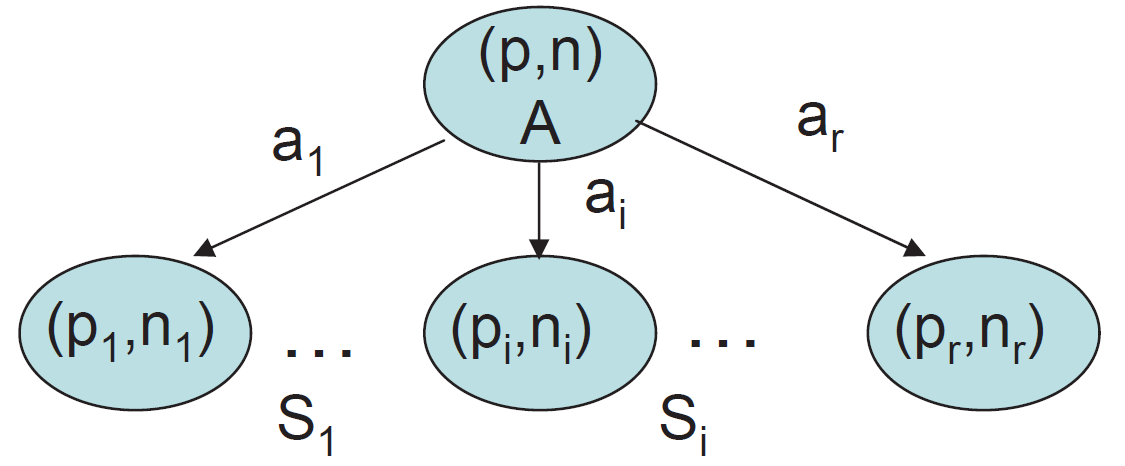
\includegraphics[width=200pt]{figures/decision-tree.png}
\caption{Esemplificazione di un albero di decisione}
\label{fig:albero-decisione}
\end{figure}

Con riferimento alla figura \ref{fig:albero-decisione}, si nota che:
\begin{itemize}
\item $S_i \cap S_j = \emptyset, \forall i \neq j$, cioè ogni sotto-albero $S_i$ è disgiunto dagli altri $S_j$ adiacenti (nello stesso livello)
\item $S_i= \lbrace e \in S | A(e) = a_i \rbrace$, per ogni esempio $e$ appartenente ad un sotto-albero $S_i$, l'attributo $A(e)$ assume sempre lo stesso valore $a_i$ (l'attributo selezionato per caratterizzare il sotto-albero $S_i$ ha valore costante in tutti i sotto-alberi figli)
\end{itemize}

\subsection{Costruzione dell'albero di decisione}
A partire da esempi pre-classificati in fase di training, il sistema genera un albero di decisione in cui $S_0$ è la radice. Ad ogni nodo $\sigma$ viene selezionato il miglior attributo $A^*$, in accordo a qualche criterio, per effettuare il test a quel nodo. Infine, si assegna il nome di una classe ad ogni nodo foglia.

L'albero può anche essere validato su un insieme di testing: si segue il cammino dalla radice ad una foglia testando ad ogni nodo il valore dell'attributo selezionato, e procedendo il cammino sul valore (o range di valori) dell'osservazione da classificare.

\subsection{Scelta dell'attributo più discriminante}
Esistono diversi criteri euristici per scegliere l'attributo più discriminante ad ogni livello, ognuno dei quali utilizza una misura specifica per massimizzare l'effetto discriminante:
\begin{itemize}
\item Massimizzazione dell'\textbf{informazione}
	\begin{itemize}
	\item entropia minima
	\item rapporto di guadagno
	\item guadagno di informazione normalizzato
	\item riduzione della lunghezza della descrizione
	\end{itemize}
\item Minimizzazione dell'\textbf{errore}
	\begin{itemize}
	\item riduzione dell'errore nel training set
	\item dissimilarità
	\item indice di diversità di Gini
	\end{itemize}
\item Massimizzazione della \textbf{significatività}, basato su statistiche varie ($\chi^2$, $G$, $\cdots$)
\end{itemize}

\subsubsection{Entropia}
\label{entropia}
L'entropia definisce la \textit{impurity} di un insieme arbitrario di dati $S$, contenente esempi positivi (in proporzione $p_+$) e negativi (in proporzione $p_-$):
\[ entropia(S) = -p_+ \log_2p_+ - p_- \log_2p_- \]
In questo modo il valore dell'entropia agli estremi è:
\begin{itemize}
\item $0$ se c'è minima entropia, ovvero se tutti gli esempi sono positivi
\item $1$ se c'è massima entropia, ovvero se gli esempi sono positivi e negativi in ugual numero
\end{itemize}
La funzione entropia relativa ad una classificazione booleana varia coma la proporzione $p_+$, cioè fra $0$ e $1$.

Più in generale, se il concetto target può assumere $c$ valori anziché $2$, la funzione entropia diventa:
\[ entropia(S) = \sum_{i=1}^c -p_i \log_2p_i \]
dove $p_i$ è la proporzione di esempi in $S$ appartenenti alla classe $i$; In questo senso, la categorizzazione booleana è una sua specializzazione a due classi.

\subsubsection{Information Gain}
\label{information-gain}
L'information gain di un attributo $A$ relativo ad un insieme di esempi $S$ è così calcolato:
\[Gain(S,A) = entropia(S) - \left[ \sum_{a \in \Lambda_A} \left( \frac{|S_a|}{|S|} \times entropia(S_a) \right) \right] \]
dove $S_a$ è il sottoinsieme di $S$ per il quale l'attributo $A$ ha valore $a$.

$Gain(S,A)$ rappresenta la \textbf{riduzione attesa in entropia} (disordine), causata dal conoscere il valore dell'attributo $A$.\\
Maggiore è la riduzione dell'entropia, maggiore è il guadagno che si ottiene selezionando $A$ come attributo discriminante.

\subsection{Considerazioni sui sistemi TDIDT}
\'E possibile passare da alberi di decisione a regole di decisione, semplicemente analizzando ogni cammino dai nodi foglia al nodo radice e generando, per ognuno, una regola in cui la scelta di uno specifico arco introduce un nuovo congiunto.

I sistemi TDIDT sono molto efficienti, e gli alberi di decisione possono trattare sia attributi a valori categorici, gestendo più archi uscenti da ogni nodo, che continui, tramite definizione di intervalli che vanno a configurarsi come categorie.

Essi sono inoltre non parametrici e non incrementali, in quanto l'introduzione di un nuovo esempio potrebbe rovinare la rigida struttura ad albero, e quindi il suo potere inferenziale.\\
Tuttavia, nel caso di dati rumorosi, potrebbero essere generati alberi di dimensioni enormi, che andrebbero quindi gestiti con opportuni algoritmi di pruning.

Altri metodi, infine, rimpiazzano i nodi foglia con distribuzioni di probabilità della classe inferita, soprattutto con numerosi esempi di apprendimento.

\subsection{C4.5}
Per apprendere regole utili a classificare appositamente una seduta di dialisi si \'e scelto di implementare il funzionamento base dell'algoritmo C4.5 di Ross Quinlan \cite{Quinlan:1993:CPM:583200} \cite{Salzberg:1994:BRC:198277.637825}, estensione del precedente ID3\cite{Mitchell:1997:ML:541177}. In questo modo risulta possibile:
\begin{itemize}
\item utilizzare la sintomatologia come attributo target (da classificare)
\item poter sfruttare i numerosi dati disponibili
\item generare un albero di decisione
\item convertire l'albero in un insieme di regole Prolog
\end{itemize}

L'implementazione del C4.5 \'e stata descritta, concettualmente e nella sua implementazione, in \ref{prolog-impl-passi-base}.

\section{Test dell'algoritmo}
Gli esempi di rilevazioni di sintomatologie a disposizione sono, purtroppo, mal distribuiti: alcune sintomatologie sono molto presenti, mentre altre sono molto rare.
Per questo motivo, e per valutare la stabilit\'a del sistema, si \'e ritenuto opportuno validare le regole generate.

\subsection{Test su algoritmi di IA}
Il processo di apprendimento per gli schemi più comuni opera in più fasi:
\begin{enumerate}
\item Costruzione della struttura base a partire dai \textbf{training data}
\item Ottimizzazione delle impostazioni sui parametri, eseguita con i \textbf{validation data}
\item Test del sistema ottenuto, tramite i \textbf{test data}
\end{enumerate}
Ovviamente training, validation e test data sono insiemi di dati completamente indipendenti.\\
A valutazione completa, infine, tutti i dati rilevati devono essere utilizzati per ricostruire un nuovo classificatore per l'utilizzo effettivo.

Non potendo disporre di un dataset molto stabile\footnote{Al momento \'e in corso un procedimento per raccogliere dati da pi\'u centri di dialisi in tutta Italia, in modo tale da disporre di un insieme di esempi pi\'u ricco e fare meno ricorso a filling-in di dati nulli. Sarebbe inoltre utile rilevare dati per razze diverse da quella caucasica, che copre l'intero \textit{set} di esempi, rendendo l'analisi di tale attributo praticamente inutile.}, tuttavia, si \'e dovuto ricorrere ad altre tecniche per realizzare un classificatore che possa essere ritenuto valido.

\subsection{K-Fold Cross-Validation}
\label{k-fold}
La \textbf{cross-validation} \'e una metodologia di test che divide l'insieme dei dati in:
\begin{itemize}
\item \textbf{training set}, di solito $\frac{9}{10}$ dei dati originali
\item \textbf{testing set}, di solito $\frac{1}{10}$ dei dati originali
\end{itemize}

Operando in questa maniera, l'insieme dei dati di test \'e sempre differente dall'insieme dei dati di \textit{training}. In generale, il processo:
\begin{enumerate}
\item Divide i dati in $k$ sotto-insiemi di dimensioni uguali.
\item Utilizza, a turno, ogni sotto-insieme per il testing, ed i rimanenti per il training.
\item Esegue, alla fine dei $k$ passi, una media delle stime di errore per ottenere una \textbf{stima di errore finale}.
\end{enumerate}

Poiché la cross-validation partiziona l'insieme degli esempi in $k$ sotto-insiemi, è chiamata anche \textbf{k-fold cross-validation}.

Il metodo standard per la valutazione è il \textbf{10-fold cross-validation}, che divide lo spazio degli esempi in $10$ sotto-insiemi, in quanto sperimentazioni estensive (ma anche dimostrazioni teoriche) hanno rilevato che $10$ è la scelta migliore di partizionamento per poter fornire una stima accurata.

\section{Implementazione in Prolog}
\label{prolog}
Il programma Prolog \'e diviso in $6$ moduli, ognuno dei quali si occupa di parti differenti del programma\footnote{Ogni regola definita nei diversi moduli \'e stata documentata. La documentazione \'e consultabile aprendo in un browser il file \texttt{doc/index.html}. Per un problema nel modulo di generazione della documentazione, i link diretti dalla \texttt{index.html} alle regole documentate non funzionano; utilizzare, invece, i collegamenti ai moduli, dai quali si pu\'o comunque accedere alla documentazione delle regole.}.

Si \'e scelto di utilizzare SWI-Prolog\cite{SWI:2014:Online} come ambiente Prolog.

\subsection{Utility}
\label{prolog-utility}
Sono stati realizzati $2$ moduli che realizzano funzioni di utilit\'a.

\subsubsection{\texttt{util.pl}}
\verb|util.pl| contiene brevi regole che implementano:
\begin{itemize}
\item timer, con avvio, lettura e stop (\verb|timer_start|, \verb|timer_get|, \verb|timer_stop|, tra gli altri)
\item formattazione di millisecondi (\verb|format_ms|) e secondi (\verb|format_s|) nel formato intellegibile \texttt{\{M\}m \{S\}s \{MS\}ms}
\item stampa a video di generiche liste di elementi o di un elemento singolo, con ritorno a capo (\verb|println|)
\item generici \textit{helper} per liste, che realizzano funzioni di minimo e massimo (\verb|list_min|, \verb|list_max|), ricerca dell'elemento pi\'u comune (\verb|list_most_common|) e dell'indice di un elemento specifico (\verb|index_of|), oltre che funzionalit\'a di aggiunta e rimozione di elementi
\item concatenazione di elementi di una lista in una stringa
\item realizzazione del logaritmo in base $2$ (\verb|log2|), utilizzato successivamente (cfr. \ref{prolog-learner}).
\end{itemize}

\subsection{Avvio del programma}
\label{prolog-main}
Il programma principale \'e definito nel modulo \verb|main.pl|, che si occupa del caricamento in memoria di tutti i file Prolog necessari e di definire il metodo \verb|main(Config, Symptom)|:
\begin{itemize}
\item \verb|Config| dichiara al programma qual \'e il file di configurazione con il quale si vuole accedere al database.\footnote{Alcuni file di configurazione di esempio sono presenti nella cartella \texttt{prolog/config}.}. Vedi \ref{prolog-database} per il l'accesso al database. Si \'e optato per un file di configurazione che contenesse tutti i parametri di connessione poich\'e la scrittura degli stessi ad ogni avvio del programma sarebbe risultata troppo verbosa.
\item \verb|Symptom| definisce l'ID del sintomo che si vuole utilizzare come esempio positivo per l'attributo target.
\end{itemize}

Entrambi i parametri supportano i meta-valori \verb|default| e \verb|ask|: \verb|default| esegue un \textit{fallback} dei parametri sul file di configurazione \texttt{prolog/config/database.properties} (si veda \ref{appendix-data} per l'importazione dei dati) e sul sintomo con ID $2$, mentre \verb|ask| imposta il programma in modo da chiedere all'utente, in maniera interattiva e quando necessario, gli stessi parametri. La figura \ref{fig:prolog-start} mostra l'avvio dell'algoritmo con il file di configurazione di default e per il sintomo $8$.

\begin{figure}[!htb]
\centering
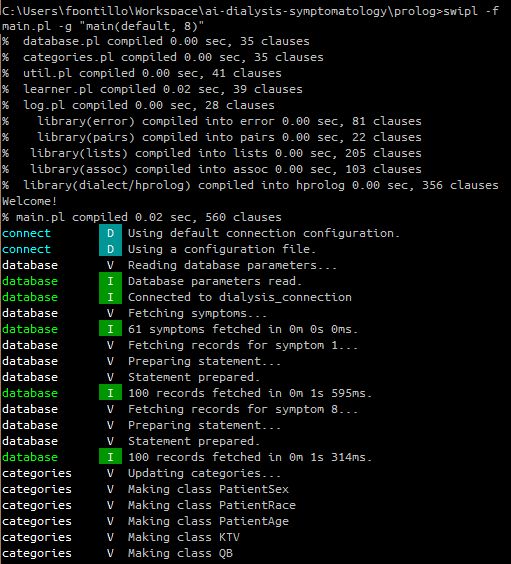
\includegraphics[width=250pt]{figures/prolog-start.png}
\caption{Avvio del programma per il sintomo $2$}
\label{fig:prolog-start}
\end{figure}

Sono anche presenti funzioni di avvio rapido: \verb|main_def/0| (che avvia il programma con parametri di default), \verb|main/0| (che avvia in modalit\'a \verb|ask|) e \verb|make_doc/0| (che genera la documentazione HTML).

Il sistema di logging implementato \'e, di default, molto verboso. Se non si vuole avere in output il dettaglio completo di ci\'o che sta avvenendo nel programma, \'e possibile utilizzare le regole messe a disposizione dal modulo di logging (vedi \ref{prolog-utility}) per settare un livello di logging meno verboso:
\begin{verbatim}
  ?- log_level(info).
\end{verbatim}

Per uscire dal programma e chiudere in maniera pulita la connessione, basta chiamare la regola \verb|out|.

\subsection{Lettura dal database}
\label{prolog-database}
Una volta letti i parametri impostati dal \verb|main| vengono eseguiti i processi di connessione e lettura dei dati utili alla generazione dell'albero di decisione.

La lettura dal database \'e possibile grazie alla libreria \verb|odbc| di SWI-Prolog \footnote{Per questa ragione, \'e necessario che sulla macchina client siano installati i driver di connessione ODBC al database target. Poich\'e i parametri sono impostati dal programma Prolog, non \'e necessario creare nessuna connessione sulla macchina.}.

\subsubsection{Connessione}
La connessione al database avviene tramite la regola \verb|connect| (nelle varianti) e i parametri nel file di configurazione impostato in precedenza: driver ODBC, indirizzo e porta, username, password e database. Se si \'e in modalit\'a \verb|ask|, il file di configurazione verr\'a chiesto all'utente, e nel caso in cui non esista viene eseguito un \textit{fallback} sul file di default.

La lettura del file \verb|.properties| \'e eseguita da
\begin{verbatim}
  read_database_params(Path, Driver, Server, 
  	Port, Database, User, Password)
\end{verbatim}
che utilizza il costrutto \verb|open_table| di SWI-Prolog per leggere i campi del file di propriet\'a e unificare con le variabili passate in input.

\subsubsection{Lettura sintomi}
Il passo successivo consiste nella lettura di tutte le possibili sintomatologie che potrebbero verificarsi nel corso di una seduta di dialisi. La regola \verb|get_symptoms/0| esegue una semplice \texttt{SELECT} sulla base di dati, ottenendo, salvando in memoria e stampando a video i sintomi.

\subsubsection{Lettura degli esempi}
La regola \verb|update_records/0| si occupa di ottenere e salvare in memoria tutti gli esempi che devono essere utilizzati per avviare il processo di apprendimento.

Poich\'e \'e necessaria la selezione sia degli esempi positivi che di quelli negativi, \verb|update_records/0| esegue lo stesso \textit{statement} di \texttt{SELECT}, opportunamente creato e preparato, andando a modificare l'ID della sintomatologia target da ottenere\footnote{La regola \verb|get_records/2| prepara lo statement all'esecuzione.}. Per lo scopo del progetto \'e stato imposto un limite di $100$ esempi positivi e $100$ esempi negativi, in modo tale da velocizzare il processo di generazione delle regole.

Il salvataggio dei record avviene andando ad asserire, nella memoria del programma Prolog, strutture del tipo:
\begin{verbatim}
  positive(ID, Attribute, Value)
  negative(ID, Attribute, Value)
\end{verbatim}
In questo modo \'e sempre possibile accedere a qualsiasi coppia attributo-valore di un esempio con uno specifico ID, sia esso positivo o negativo.

\'E stata realizzata anche la regola
\begin{verbatim}
  example(Type, ID, Attribute, Value)
\end{verbatim}
dove \verb|Type| pu\'o essere \verb|positive| o \verb|negative|. Tramite questa modalit\'a \'e possibile accedere a tutti gli esempi prelevati dalla base di dati. Sono presenti, inoltre, regole di conteggio e di verifica di esistenza (cfr. documentazione HTML).

\subsection{Suddivisione attributi in range}
\label{prolog-categories}
Gli attributi dei dati di esempio possono essere numerici (a virgola mobile) o categorici, ma in ogni caso sono identificati da un numero. Essi sono stati dichiarati esplicitamente tramite la clausola \verb|data_type(Attribute, Type)|, che definisce quindi la tipologia per ogni attributo.

Per ogni attributo, quindi, si \'e avviato un processo di suddivisione (\verb|update_categories/0| e \verb|make_class/2|) in pi\'u \textit{range}, definite dal predicato \verb|class/2|:
\begin{itemize}
\item gli attributi di tipo \verb|category| sono gi\'a automaticamente partizionati, per cui una classe di tipo categorico avr\'a i range corrispondenti a tutti i valori di categoria
\item ogni attributo di tipo \verb|number| \'e stato suddiviso in $10$ range di dimensioni uguali\footnote{L'approccio utilizzato \'e semplicistico, quindi passibile di miglioramento, vedi \ref{sviluppi-futuri}.}
\end{itemize}

Il modulo \verb|categories| contiene, nelle sue due varianti, il predicato \verb|is_in_range|, che risulta soddisfatto solo se il valore (numerico o categorico che sia) rientra nel \textit{range} specificato.

\subsection{Apprendimento e test}
\label{prolog-learner}
Dopo aver generato le categorie, \'e possibile avviare il processo (iterativo e ricorsivo) di apprendimento e test tramite la regola \verb|learn_please/0|.

Lo scopo di questa fase \'e di generare due tipi di regole:
\begin{itemize}
\item \verb|is_positive(ID, LearningStep| determina se, secondo le regole generate ad un certo passo \verb|LearningStep|, un esempio con un determinato \verb|ID| \'e ritenuto un positivo.
\item \verb|test_step(LearningStep, StepData)| restituisce diverse misure relative allo step specificato, fra cui ``true positive rate'', ``false positive rate'', F-Measure, ecc.
\end{itemize}

L'iterazione principale del processo di apprendimento \'e definita dal $k$\textit{-fold cross-validation}:
\begin{enumerate}
\item L'insieme degli esempi (positivi e negativi) viene diviso in $k$ sottoinsiemi. Per lo scopo del progetto, si \'e impostato un $k$ fisso a $10$.
\item\label{apprendimento-k-fold} Ad ogni iterazione, un sottoinsieme viene messo da parte per la fase di test, mentre gli altri $9$ concorrono all'apprendimento vero e proprio.
\item L'apprendimento viene avviato, generando regole di tipo \verb|is_positive/2|.
\item Viene eseguito il test con l'insieme di esempi selezionato, generando regole di tipo \verb|test_step/2|.
\item Si itera dal punto \ref{apprendimento-k-fold} fino ad esaurimento dei $k$ \textit{fold} creati.
\item Tutte le regole create vengono unite in un unico insieme, rimuovendo i duplicati.
\end{enumerate}

L'apprendimento, per ogni fase, \'e avviato da \verb|learn(Step)|.

\subsubsection{Suddivisione in fold}
La suddivisione in $k$ fold distinti viene eseguita, ad ogni passo, dal predicato \verb|split_examples/2| (vedi figura \ref{fig:prolog-k-fold} per un esempio), che asserisce in memoria alcune liste di \verb|ID| di esempi. Tali liste sono poi utilizzate nel filtraggio, quando richiesto, degli esempi in \textit{training} e \textit{testing}.

Nei primi test del programma, si \'e notato un bassissimo livello di distribuzione degli esempi nei diversi fold di ogni esecuzione, per cui i primi \textit{run} avevano un bassissimo livello di \textit{error rate} (spesso $0$), che cresceva con l'aumentare dell'indice del passo.\\
Ci\'o era dovuto non alla generazione di regole ottimali, ma al fatto che gli esempi positivi venivano selezionati, da Prolog, sempre dopo quelli negativi, comportando un insieme di test composto, ai primi passi, da molti esempi positivi (mentre erano pochi o nulli alla fine) e da pochi negativi (mentre erano molti alla fine).

Si \'e pertanto reso necessario ``forzare'' una distribuzione pi\'u o meno uniforme andando a dividere i \textit{set} di positivi e negativi in \textit{fold} separati, che sono poi stati comunque accorpati in due liste complessive, visionabili a fine step con:
\begin{verbatim}
  ?- train_examples(TrainExamples).
  ?- test_examples(TestExamples).
\end{verbatim}

Il filtraggio degli esempi viene poi eseguito da \verb|test_example/4| e \verb|train_example/4| e da altre regole derivate.

\begin{figure}[!htb]
\centering
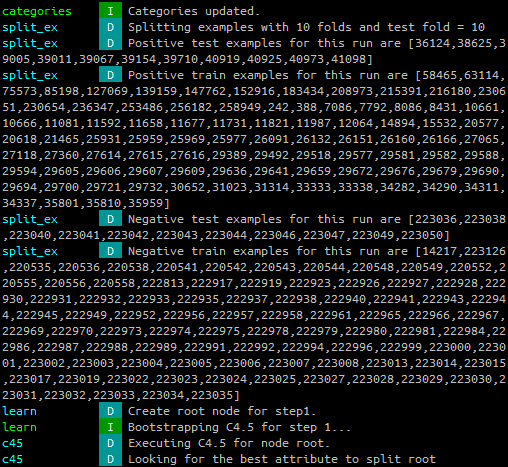
\includegraphics[width=250pt]{figures/prolog-k-fold.png}
\caption{Suddivisione in $10$ fold, al passo $9$: il secondo \textit{fold} viene selezionato per il test, gli esempi rimanenti come training set}
\label{fig:prolog-k-fold}
\end{figure}

\subsubsection{Apprendimento}
L'implementazione dell'algoritmo C4.5 \'e abbastanza diretta, e si compone di passi ricorsivi che iniziano dalla generazione di un nodo radice.

In generale, tutti i nodi dell'albero di decisione sono cos\'i composti:
\begin{verbatim}
  node(Name, Parent, SplitAttribute, SplitRange)
\end{verbatim}
dove:
\begin{itemize}
\item \verb|Name| corrisponde ad un generico nome, che non \'e detto sia univoco, per il nodo. Genericamente, il nome del nodo \'e composto dall'attributo su cui il nodo genitore \'e stato suddiviso e una descrizione testuale del \textit{range} che il nodo rappresenta.
\item \verb|Parent| rappresenta il \verb|node/4| genitore; per questa ragione, ogni nodo pu\'o essere identificato univocamente dalla coppia \verb|(Name, Parent)|.
\item \verb|SplitAttribute| \'e l'attributo su cui \'e stato eseguito lo \textit{split} per il livello corrente dell'albero.
\item \verb|SplitRange| \'e il range dell'attributo di \textit{split} che il nodo corrente espande.
\end{itemize}

Il nodo radice, non potendo derivare nessuno dei precedenti parametri, ha come valori l'atomo \verb|root|, per semplicit\'a.

I nodi foglia dell'albero sono identificati dalla regola:
\begin{verbatim}
  node_label(Node, Value)
\end{verbatim}
che specifica che un nodo dell'albero \'e terminale e identifica tutti gli esempi rimanenti come appartenenti a uno specifico range della classe target.

\paragraph{Passi base}
\label{prolog-impl-passi-base}
Il processo ricorsivo dell'algoritmo C4.5 inizia, quindi, dal nodo \verb|root|. Ogni chiamata alla regola \verb|c45/3| richiede che siano istanziate le seguenti variabili:
\begin{itemize}
\item \verb|Node| deve essere un \verb|node/4|, e deve contenere le informazioni sul nodo che si vuole suddividere in pi\'u \textit{split}.
\item \verb|Examples| \'e una lista di \verb|ID| di esempi, ovvero quei dati che devono essere processati al passo corrente.
\item \verb|Attributes| è la lista di nomi di attributi che non sono ancora stati selezionati per lo \textit{split}.
\end{itemize}

Ovviamente il primo passo vedr\'a \verb|Examples| contenere tutti gli esempi e \verb|Attribute| tutti gli attributi.

Il primo controllo che viene eseguito da \verb|c45/3| verifica se tutti gli \verb|Examples| appartengono gi\'a ad un'unica classe target, ovvero se tutti gli esempi hanno una stessa sintomatologia. In caso affermativo:
\begin{enumerate}
\item Si asserisce in memoria un \verb|node_label/2| che dichiara che il nodo corrente ha come unica classe target quella rilevata.
\item Il nodo corrente non viene pi\'u espanso.
\item Viene restituito il controllo al chiamante, ovvero il livello (nodo) superiore.
\end{enumerate}

Se tale controllo non \'e soddisfatto, se ne fa un altro relativamente alla lista di attributi rimanenti; se la lista \'e vuota, infatti, si segue lo stesso procedimento per il controllo precedente, con l'unica differenza che il range associato a \verb|node_label| \'e quello relativo al valore pi\'u comune fra gli esempi rimanenti.

Se nessuna delle verifiche precedenti porta a risultati, il nodo corrente dovr\'a essere nuovamente diviso in \textit{split}. Il processo, allora, prosegue con:
\begin{enumerate}
\item Selezione del migliore attributo.
\item Split sui range dell'attributo selezionato.
\item Chiamata ricorsiva a \verb|c45/3|.
\end{enumerate}

\paragraph{Attributo migliore}
\label{apprendimento-attributo-migliore}
Per poter decidere quale, fra gli attributi rimanenti, costituisce il migliore ai fini del processo di apprendimento, si \'e deciso di utilizzare la misura dell'~\textit{information gain} (vedi \ref{information-gain}), che a sua volta si basa fortemente sull'entropia (vedi \ref{entropia}). Un esempio di esecuzione \'e visibile in figura \ref{fig:prolog-best-attribute}, dove viene scelto \verb|PatientSex| poich\'e possiede il massimo \textit{information gain}.

L'entropia viene calcolata dalla regola \verb|entropy/2|, che utilizza i \verb|train_example/4|; l'\textit{information gain}, invece, viene calcolato da \verb|info_gain/3|, che si basa sul calcolo dell'entropia e che somma, per ogni range dell'attributo $A$, il valore restituito da \verb|partial_info_gain/4|:
\[\frac{|S_a|}{|S|} \times entropia(S_a)\]

\begin{figure}[!htb]
\centering
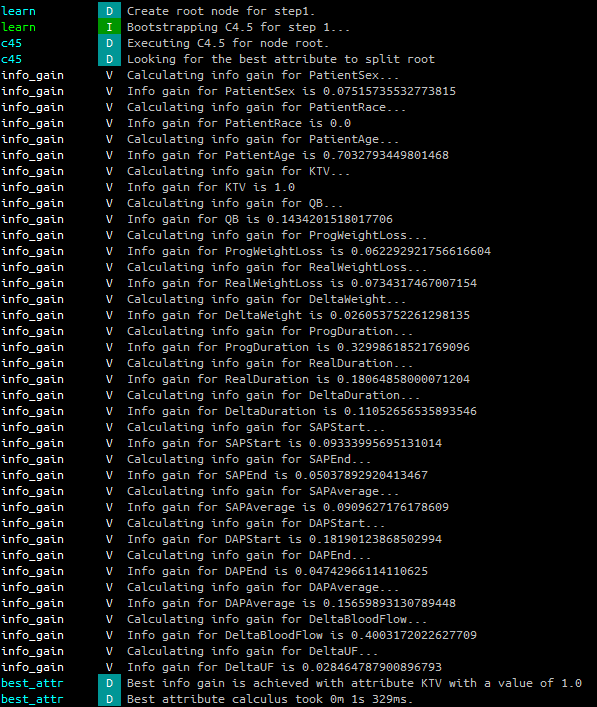
\includegraphics[width=250pt]{figures/prolog-best-attribute.png}
\caption{Scelta dell'attributo migliore secondo l'\textit{information gain}}
\label{fig:prolog-best-attribute}
\end{figure}

Si noti che la misura dell'\textit{information gain} equivale all'entropia quando tutti i sottoinsiemi selezionati dalle coppie attributo-range:
\begin{itemize}
\item sono vuoti, rendendo $|S_a|=0$
\item alternativamente se tutti gli esempi appartengono a una sola delle due classi (positivo o negativo), cio\'e se il sottoinsieme selezionato ha minima entropia ($0$)
\end{itemize}

\paragraph{Split sui range}
Dopo aver calcolato l'\textit{information gain} per tutti gli attributi, si seleziona quello con la misura pi\'u elevata e si ottengono tutti i suoi \textit{range}.

\paragraph{Creazione nodi figli}
Per ogni range dell'attributo si crea un nuovo nodo avente come nome il template seguente:
\begin{verbatim}
  [ Attribute : range(Inizio, Fine) ]
\end{verbatim}
Si chiama, infine, la regola \verb|c45| con parametri:
\begin{itemize}
\item \verb|Node| il nodo appena creato
\item \verb|ParentNode| il nodo correntemente in analisi e in ingresso al passo corrente
\item \verb|Attributes| l'insieme di attributi in ingresso al passo corrente, eccetto l'attributo su cui \'e stato eseguito lo \textit{split}
\end{itemize}

\paragraph{Terminazione locale}
Quando non ci sono pi\'u esempi da analizzare, o gli attributi su cui eseguire lo \textit{split} sono terminati, l'algoritmo termina, avendo prodotto un albero di decisione completo.

\begin{figure}[!h]
\centering
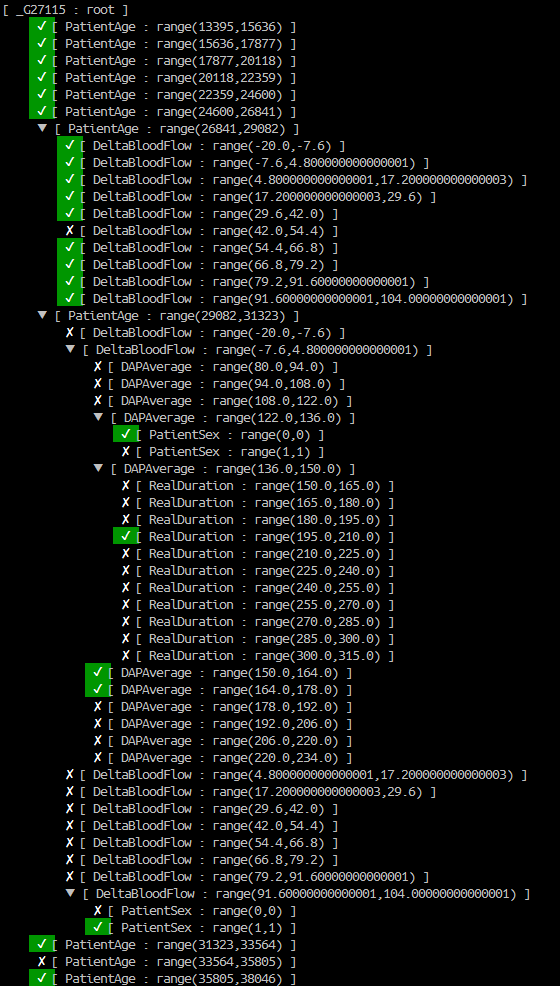
\includegraphics[width=250pt]{figures/prolog-le-tree.png}
\caption{Stampa dell'albero generato al passo corrente}
\label{fig:prolog-le-tree}
\end{figure}

Viene quindi stampata a video, richiamando la regola \verb|print_le_tree/0|, una rappresentazione grafica e formattata dell'albero di decisione prodotto, in cui ogni elemento foglia (positivo) avr\'a un check verde (vedi figura \ref{fig:prolog-le-tree}).

\subsubsection{Generazione di regole}
Una volta appreso l'albero di decisione ad uno specifico passo $i$, il programma genera le regole \verb|is_positive/2| andando a risalire l'albero di decisione da ogni nodo foglia positivo \verb|node_label/2|, e aggiungendo in lista una condizione di appartenenza dell'attributo su cui il nodo \'e stato ``splittato'' al range del nodo stesso\footnote{Vengono generate regole per i soli nodi foglia positivi.}.

La regola principale che si occupa della generazione delle regole \'e \verb|gen_all_the_rulez/1|, che chiama ricorsivamente \verb|gen_rule/2| per ogni nodo foglia.

\subsubsection{Test del passo}\label{test-step}
Dopo la generazione delle regole al passo $i$, si esegue un processo di test, che asserisce in memoria (nel predicato \verb|test_step/2|) diverse informazioni relative al passo in analisi.

I predicati \verb|p/1| e \verb|n/1| esplicitano, banalmente, il numero di positivi e negativi analizzati al passo corrente. Tali valori sono utilizzati, insieme ad altri calcoli, per generare anche:
\begin{itemize}
\item \verb|tn(TrueNegatives)|, ovvero la quantit\'a di negativi non classificati (ovvero classificati come negativi, poich\'e il sistema genera regole per la sola classe positiva)
\item \verb|fn(FalseNegatives)|, cio\'e i positivi erroneamente classificati come negativi
\item \verb|tp(TruePositives)|, i positivi correttamente classificati
\item \verb|fp(FalsePositives)|, cio\'e i negativi erroneamente classificati come positivi
\item \verb|tp_rate(TruePosRate)|, la proporzione dei veri positivi su tutti i positivi
\item \verb|tn_rate(TrueNegRate)|, la proporzione dei veri negativi su tutti i negativi
\item \verb|fp_rate(FalsePosRate)|, la proporzione dei falsi positivi su tutti i negativi
\item \verb|fn_rate(FalseNegRate)|, la proporzione dei falsi negativi su tutti i positivi
\end{itemize}

Inoltre, vengono calcolate anche \textit{precision} e \textit{recall}:
\[
\begin{cases}
precision = \frac{tp}{tp+fp} \\
recall = \frac{tp}{tp+fn}
\end{cases}
\]
Tali valori vengono esposti, nella lista restituita da \verb|test_step/2|, come \verb|precision(Precision)| e \verb|recall(Recall)|.

Infine, viene calcolata anche la $F_1\textnormal{-}Measure$, equivalente a:
\[ F_1\textnormal{-}Measure = \frac{2*precision*recall}{precision+recall} \]

\subsection{Terminazione dell'apprendimento}
Una volta che tutti i $k$ cicli di apprendimento-test sono terminati, il programma termina l'esecuzione tramite alcuni passi finali.

\subsubsection{Generazione regole}
\label{unione-regole}
Tutte le regole generate ai diversi passi vengono inglobate in un unico insieme di regole, e riasserite come \verb|final_positive(ID, ListaPassi|), dove \verb|ListaPassi| \'e la lista degli indici dei passi che hanno generato quella regola.

Il metodo che si occupa di unire le regole in un insieme singolo \'e \verb|purge_rules/0| che, avvalendosi dei predicati \verb|clause/2| e \verb|bagof/3|, ricerca tutti i corpi delle regole \verb|is_positive/2| e li unisce, rimuovendo i duplicati.

\subsubsection{Test finale}
Una volta unite le regole, queste vengono applicate all'\textbf{intero insieme di esempi}, in modo da validare in maniera completa tutto il processo di apprendimento. Tale passo si rivela importante soprattutto nel caso in cui l'insieme degli esempi di partenza \'e molto piccolo.

Il test asserisce, in memoria Prolog, il fatto \verb|test_final/1|, che contiene le stesse informazioni presenti in \verb|test_step/2| (cfr. \ref{test-step}).

\subsubsection{Stampa report}
Tutte le informazioni vengono quindi stampate a schermo da \verb|print_report/0| (vedi figura \ref{fig:prolog-report}) che, avvalendosi del sistema di logging implementato, mostra sul livello \verb|info|:
\begin{itemize}
\item una ricapitolazione di tutte le informazioni asserite ad ogni esecuzione
\item la media delle singole esecuzioni\footnote{Come gi\'a detto, la media potrebbe essere poco indicativa per dataset molto piccoli.}
\item l'esecuzione del test finale
\end{itemize}

\begin{figure}[!h]
\centering
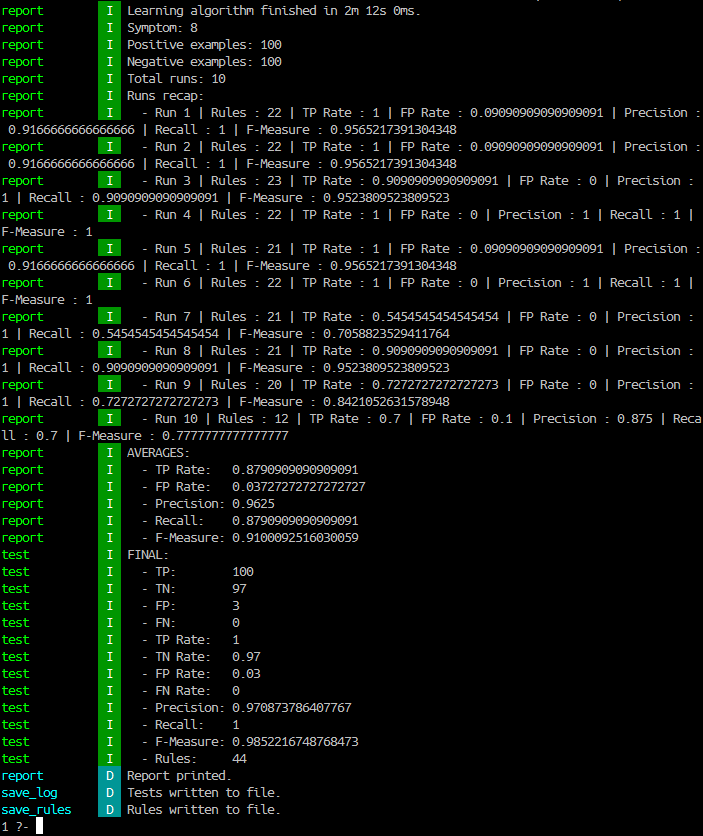
\includegraphics[width=250pt]{figures/prolog-report.png}
\caption{Stampa del report di fine processo}
\label{fig:prolog-report}
\end{figure}

\subsubsection{Salvataggio log e regole}

Al termine di ogni processo di apprendimento viene creato un file, \verb|runs/log_{ID}.csv|\footnote{Per la creazione dei file di log, \'e necessario che la cartella \verb|runs| esista gi\'a.} contenente, per ogni esecuzione: il sintomo, il passo, il numero di regole generate e l'error rate; infine, il file riporta il tempo di esecuzione in secondi, il numero totale di esempi positivi presenti, il numero totale di regole generate e l'errore medio complessivo.

Inoltre, tutte le regole unite alla fine dell'apprendimento (vedi \ref{unione-regole}) vengono salvate nel file \verb|runs/rules_{ID}.pl|\footnote{Per la verifica delle regole \'e necessario che sia caricato in memoria Prolog anche la regola \verb|check_condition_list/2|, che serve ad eseguire il \textit{matching} dei range descritti dalla regole generate.}, ad esempio:
\begin{verbatim}
final_positive(A, [1, 2, 3, 4, 5, 6, 7, 8, 9, 10]) :-
	check_condition_list(A,
			     
			     [ condition('PatientAge',
					 range(22231.000000000004,
					       24032.200000000004))
			     ]).
\end{verbatim}

\section{Risultati}
Il programma \'e stato eseguito su $9$ sintomi target distinti e con un diverso numero di esempi positivi\footnote{La macchina utilizzata per il test ha le seguenti caratteristiche:
\begin{itemize}
\item CPU Intel i7-4500U @ 1.80GHz
\item 8GB RAM DDR3
\item Samsung SSD EVO 840 250GB (fino a 540 MB/s in lettura, fino a 520 MB/s in scrittura)
\item Windows 8.1 x64
\end{itemize}}.

\subsection{Prime considerazioni}

La tabella \ref{table:risultati-ktv-qb-test} mostra un breve riepilogo dei risultati dei test (finali) eseguiti sull'intero dataset, per i sintomi $2$, $3$, $4$ ,$5$, $6$, $7$, $8$, $9$, $10$. I valori mostrati in tabella\footnote{Tutti i report delle esecuzioni, con tutti i valori calcolati, anche parziali, si trovano nella cartelle \verb|runs/| e \verb|runs_ktv_qb/|.} sono:
\begin{itemize}
\item \verb|ID| del sintomo analizzato
\item Tempo di esecuzione, in secondi, del processo di apprendimento e di test con la $10$\textit{-fold cross-validation}
\item Numero di esempi positivi analizzati (i negativi sono sempre $100$)
\item Numero di regole (differenti) generate
\item \textit{True Positive Rate}, ovvero il rapporto dei veri positivi sul numero dei positivi
\item Misura di \textit{precision}
\item Misura di \textit{recall}
\item La \textit{F-Measure}
\end{itemize}

\begin{table}[h]
\centering
\begin{tabular}{|c|c|c|c|c|c|c|c|} \hline
& \textbf{T} &\textbf{+} &\textbf{\#Reg} &\textbf{TPR} &\textbf{Prec.} &\textbf{Rec.} &\textbf{F-M.}  \\ \hline \hline
$2$	&$66$	&$19$	&$2$	&$0.053$	&$0.5$		&$0.053$	&$0.095$	\\ \hline
$3$ &$33$	&$56$	&$2$	&$0.179$	&$0.909$	&$0.179$	&$0.299$	\\ \hline
$4$ &$12$	&$7$	&$0$	&$0$		&$0$		&$0$		&$0$		\\ \hline
$5$ &$50$	&$100$	&$10$	&$0.79$		&$0.94$		&$0.79$		&$0.859$	\\ \hline
$6$ &$15$	&$34$	&$0$	&$0$		&$0$		&$0$		&$0$		\\ \hline
$7$ &$11$	&$1$	&$1$	&$1$		&$1$		&$1$		&$1$		\\ \hline
$8$ &$33$	&$100$	&$1$	&$0.01$		&$1$		&$0.01$		&$0.0198$	\\ \hline
$9$	&$16$	&$5$	&$14$	&$1$		&$0.833$	&$1$		&$0.909$	\\ \hline
$10$&$25$	&$59$	&$0$	&$0$		&$0$		&$0$		&$0$		\\
\hline\end{tabular}
\caption{Risultati dei test su $9$ sintomi, includendo fra gli attributi sia \texttt{KTV} che \texttt{QB}}
\label{table:risultati-ktv-qb-test}
\end{table}

Durante l'esecuzione del programma sui vari sintomi, per\'o, si \'e notato che gli attributi \verb|KTV| e \verb|QB| condizionavano enormemente le regole prodotte, poich\'e venivano scelti molto spesso come attributo con maggior \textit{information gain}.

\subsection{Eliminazione di KTV e QB}
\label{risultati-no-ktv-qb}
Si \'e quindi effettuata un'altra esecuzione del programma, sugli stessi sintomi, eliminando gli attributi \verb|KTV| e \verb|QB| dall'analisi. I risultati di tale esecuzione sono riportati in tabella \ref{table:risultati-test}, dalla quale risultano evidenti alcune situazioni.

Innanzitutto si nota che con un \textbf{basso numero di esempi positivi} vengono generate numerose regole. Tuttavia, bisogna considerare che alcune regole potrebbero essere superflue, ovvero hanno senso di esistere esclusivamente all'interno di uno specifico insieme di \textit{fold} considerato ad un passo; potrebbe capitare, infatti, che esistano regole pi\'u generali che coprano almeno gli stessi esempi di una o pi\'u regola specifica, senza introdurre grosse variazioni di precisione\footnote{In tal senso, sarebbe utile estendere il programma con una funzionalit\'a di pulizia delle regole superflue.}.

Avendo a disposizione un \textbf{elevato numero di esempi positivi} (si vedano i sintomi $3$, $5$ e $8$), invece, la proporzione $regole/positivi$ si mantiene intorno allo $0.5$. Anche in questo caso, comunque, si deve fare la stessa considerazione precedente, ovvero che alcune regole potrebbero essere eliminate senza grossi problemi.

Altre regole, invece, potrebbero essere eliminate andando ad accorpare range ``adiacenti'' (immediatamente successivi) di attributi si trovano in alto nell'albero di decisione generato.

\begin{table}[h]
\centering
\begin{tabular}{|c|c|c|c|c|c|c|c|} \hline
& \textbf{T} &\textbf{+} &\textbf{\#Reg} &\textbf{TPR} &\textbf{Prec.} &\textbf{Rec.} &\textbf{F-M.}  \\ \hline \hline
$2$	&$90$	&$19$	&$22$	&$1$	&$0.826$	&$1$	&$0.905$	\\ \hline
$3$ &$90$	&$56$	&$26$	&$1$	&$0.875$	&$1$	&$0.933$	\\ \hline
$4$ &$25$	&$7$	&$23$	&$1$	&$0.636$	&$1$	&$0.778$	\\ \hline
$5$ &$358$	&$100$	&$60$	&$1$	&$0.909$	&$1$	&$0.952$	\\ \hline
$6$ &$220$	&$34$	&$49$	&$1$	&$0.829$	&$1$	&$0.907$	\\ \hline
$7$ &$12$	&$1$	&$1$	&$1$	&$1$		&$1$	&$1$		\\ \hline
$8$ &$132$	&$100$	&$44$	&$1$	&$0.971$	&$1$	&$0.985$	\\ \hline
$9$	&$14$	&$5$	&$15$	&$1$	&$0.833$	&$1$	&$0.909$	\\ \hline
$10$&$51$	&$59$	&$25$	&$1$	&$0.967$	&$1$	&$0.983$	\\
\hline\end{tabular}
\caption{Risultati dei test su $9$ sintomi, escludendo dagli attributi sia \texttt{KTV} che \texttt{QB}}
\label{table:risultati-test}
\end{table}

\subsection{Altri sistemi}
Lo stesso dataset \'e stato sottoposto ad altri sistemi di apprendimento automatico, in modo tale da poter valutare ci\'o che \'e stato realizzato, paragonandolo ad algoritmi ben pi\'u collaudati.

\subsubsection{Weka}
Il tool di Data Mining utilizzato \'e Weka\cite{Weka:2014:Online}, che mette a disposizione numerosi algoritmi pre-implementati per la classificazione e generazione di alberi di decisione (e regole).\\
Sono stati testati $3$ diversi algoritmi sul sintomo target $8$: J48, J48Graft e ConjunctiveRule.

Per l'importazione degli esempi \'e stata eseguita la query:
\begin{verbatim}
(SELECT 
  `PATIENT_SEX`, `PATIENT_RACE`, `PATIENT_AGE`,
  `PROG_WEIGHT_LOSS`, `REAL_WEIGHT_LOSS`,
  `DELTA_WEIGHT`,  `PROG_DURATION`, `REAL_DURATION`,
  `DELTA_DURATION`, `SAP_START`, `SAP_END`,
  `AVG_SAP`, `DAP_START`, `DAP_END`, `AVG_DAP`, 
  `BLOOD_VOLUME`,  `DELTA_BLOOD_FLOW`, 
  `DELTA_UF`, `SYMPTOM_ID`
FROM `patient_dialysis_symptom_for_analysis`
WHERE
  `SYMPTOM_ID` = 1 ORDER BY `SCORE` DESC LIMIT 100)
UNION
(SELECT
  `PATIENT_SEX`, `PATIENT_RACE`, `PATIENT_AGE`,
  `PROG_WEIGHT_LOSS`, `REAL_WEIGHT_LOSS`,
  `DELTA_WEIGHT`,  `PROG_DURATION`, `REAL_DURATION`,
  `DELTA_DURATION`, `SAP_START`, `SAP_END`,
  `AVG_SAP`, `DAP_START`, `DAP_END`, `AVG_DAP`, 
  `BLOOD_VOLUME`,  `DELTA_BLOOD_FLOW`, 
  `DELTA_UF`, `SYMPTOM_ID`
FROM `patient_dialysis_symptom_for_analysis`
WHERE
  `SYMPTOM_ID` = 8 ORDER BY `SCORE` DESC LIMIT 100)
\end{verbatim}

Una volta importati i dati del dataset di esempio in Weka Explorer (si veda \ref{appendix-weka} per una guida all'importazione e trasformazione), si possono andare a selezionare gli algoritmi da applicare.

\paragraph{J48}
J48 è un'implementazione in Java di C4.5 per Weka che opera applicando, all'albero di decisione generato, tecniche di \textit{pruning} per semplificarne la descrizione.

Lasciando i parametri di default in Weka, selezionando la $10$\textit{-fold cross-validation} come modalit\'a di test e avviando la classificazione per il sintomo target $8$, sono stati ottenuti i risultati mostrati in tabella \ref{table:risultati-j48}.

L'output di esecuzione restituito\footnote{L'output non \'e completo; per l'output completo, vedere il file \verb|weka/|} \'e il seguente:

\begin{verbatim}
=== Classifier model (full training set) ===

J48 pruned tree
------------------

PATIENT_AGE <= 29067: 8 (88.0/1.0)
PATIENT_AGE > 29067
|   PATIENT_AGE <= 30141
|   |   DAP_START <= 79: 1 (93.0/1.0)
|   |   DAP_START > 79
|   |   |   DELTA_BLOOD_FLOW <= 12: 8 (5.0/1.0)
|   |   |   DELTA_BLOOD_FLOW > 12: 1 (6.0)
|   PATIENT_AGE > 30141: 8 (8.0)

Number of Leaves  :   5

Size of the tree :  9


Time taken to build model: 0 seconds

=== Stratified cross-validation ===
=== Summary ===

Correctly Classified Instances   189  94.5 %
Incorrectly Classified Instances 11   5.5  %
\end{verbatim}

\begin{table}[h]
\centering
\begin{tabular}{|r|l|} \hline
\multicolumn{2}{|c|}{\textbf{J48}} \\ \hline \hline 
\textbf{T} & $0$ \\ \hline
\textbf{+} & $100$ \\ \hline
\textbf{\#Reg} & $3$\\ \hline
\textbf{TPR} & $0.94$ \\ \hline
\textbf{Precision} & $0.949$ \\ \hline
\textbf{Recall} & $0.94$ \\  \hline
\textbf{F-Measure} & $0.945$ \\
\hline\end{tabular}
\caption{Risultato di esecuzione con J48}
\label{table:risultati-j48}
\end{table}

A fronte di un tempo di esecuzione di gran lunga inferiore (praticamente nullo), precision e recall non differiscono di molto:
\[
\begin{cases}
precision_m = 0.971 \\
recall_m = 1 \\
fmeasure_m = 0.985
\end{cases}
\mbox{vs}
\begin{cases}
precision_{j48} = 0.949 \\
recall_{j48} = 0.94 \\
fmeasure_{j48} = 0.945
\end{cases}
\]

\paragraph{J48 Graft} J48 Graft \'e un algoritmo incluso in Weka che genera un albero di decisione con lo stesso algoritmo di J48, ma applicando la tecnica del \textit{grafting}\cite{Webb1999}, ovvero cercando di aggiungere, dove necessario, nuovi nodi all'albero prodotto per cercare di ridurre l'errore predittivo.

Utilizzando lo stesso dataset precedente e la stessa modalit\'a di testing con $10$-fold cross-validation, l'output principale ottenuto \'e il seguente:
\begin{verbatim}
=== Classifier model (full training set) ===

J48graft pruned tree
------------------

PATIENT_AGE <= 29067: 8 (88.0/1.0)
PATIENT_AGE > 29067
|   PATIENT_AGE <= 30141
|   |   DAP_START <= 79: 1 (93.0/1.0)
|   |   DAP_START > 79
|   |   |   DELTA_BLOOD_FLOW <= 12: 8 (5.0/1.0)
|   |   |   DELTA_BLOOD_FLOW > 12: 1 (6.0)
|   PATIENT_AGE > 30141: 8 (8.0)

Number of Leaves  :   5

Size of the tree :  9


Time taken to build model: 0.01 seconds

=== Stratified cross-validation ===
=== Summary ===

Correctly Classified Instances   187  93.5 %
Incorrectly Classified Instances 13   6.5  %
\end{verbatim}

L'albero di decisione generato, e le misurazioni complete mostrate in tabella \ref{table:risultati-j48-graft} non indicano alcuna differenza con J48.

\begin{table}[h]
\centering
\begin{tabular}{|r|l|} \hline
\multicolumn{2}{|c|}{\textbf{J48 Graft}} \\ \hline \hline 
\textbf{T} & $0.01$ \\ \hline
\textbf{+} & $100$ \\ \hline
\textbf{\#Reg} & $3$\\ \hline
\textbf{TPR} & $0.92$ \\ \hline
\textbf{Precision} & $0.948$ \\ \hline
\textbf{Recall} & $0.92$ \\  \hline
\textbf{F-Measure} & $0.934$ \\
\hline\end{tabular}
\caption{Risultato di esecuzione con J48 Graft}
\label{table:risultati-j48-graft}
\end{table}

\paragraph{Conjunctive Rule}
Un output pi\'u simile a quello ottenuto dal programma realizzato \'e restituito dall'algoritmo Conjunctive Rule di Weka, che genera un insieme di regole composte da un antecedente (il corpo) di clausole in congiunzione ed un sequente (la testa) che corrisponde al valore classificato.\\
Anche Conjunctive Rule calcola la misura dell'\textit{information gain} del corpo della regola generata ed esegue il \textit{pruning} in base al numero delle clausole presenti. Per la classificazione, l'informazione relativa al corpo della regola generata \'e la media pesata delle entropie degli esempi coperti dalla regola e di quelli non coperti.

L'esecuzione di Conjunctive Rule sul solito dataset ha prodotto le misure in tabella \ref{table:risultati-conjunctive-rule} e il seguente output:
\begin{verbatim}
=== Classifier model (full training set) ===

Single conjunctive rule learner:
--------------------------------
(PATIENT_AGE <= 29653.5) => SYMPTOM_ID = 8

Class distributions:
Covered by the rule:
1 8 
0 1 

Not covered by the rule:
1 8 
0.893333  0.106667  

Time taken to build model: 0.21 seconds

=== Stratified cross-validation ===
=== Summary ===

Correctly Classified Instances   185  92.5 %
Incorrectly Classified Instances 15   7.5  %
\end{verbatim}

\begin{table}[h]
\centering
\begin{tabular}{|r|l|} \hline
\multicolumn{2}{|c|}{\textbf{Conjunctive Rule}} \\ \hline \hline 
\textbf{T} & $0.21$ \\ \hline
\textbf{+} & $100$ \\ \hline
\textbf{\#Reg} & $1$\\ \hline
\textbf{TPR} & $0.87$ \\ \hline
\textbf{Precision} & $0.978$ \\ \hline
\textbf{Recall} & $0.87$ \\  \hline
\textbf{F-Measure} & $0.921$ \\
\hline\end{tabular}
\caption{Risultato di esecuzione con Conjunctive Rule}
\label{table:risultati-conjunctive-rule}
\end{table}

A fronte degli stessi esempi di training, quindi, Conjunctive Rule ha generato una sola regola, mantenendo elevata la precisione a discapito del \textit{recall}, comportando un maggior numero di falsi negativi (mancate classificazioni).
\[
\begin{cases}
precision_m = 0.971 \\
recall_m = 1 \\
fmeasure_m = 0.985
\end{cases}
\mbox{vs}
\begin{cases}
precision_{cr} = 0.978 \\
recall_{cr} = 0.87 \\
fmeasure_{cr} = 0.921
\end{cases}
\]

Andando a confrontare le regole generate dal sistema realizzato e la regola generata da Conjunctive Rule, si trova qualche disaccordo. Ad esempio:
\begin{verbatim}
final_positive(A, [1, 2, 3, 4, 5, 6, 7, 8, 10]) :-
	check_condition_list(A,
			     [condition('PatientAge', range(35805, 38046))]).
\end{verbatim}
\'e chiaramente opposta a:
\begin{verbatim}
(PATIENT_AGE <= 29653.5) => SYMPTOM_ID = 8
\end{verbatim}

Tra l'altro, la regola in esempio \'e stata generata in pi\'u passi di apprendimento, con l'unica eccezione il passo in cui tutti gli esempi che la generavano si trovavano, evidentemente, nel sottoinsieme di testing.

\subsubsection{BayesDB}
BayesDB\cite{BayesDB:2014:Online} è un ``database di tabelle bayesiane che permette di inferire le probabili implicazioni dei dati tabulati, con la stessa facilit\'a con cui si chiedono i dati ad un database SQL''. \'E un tool per inferenze molto recente, sviluppato dal MIT in collaborazione con DARPA e Google.

BayesDB, a partire da una tabella con qualsiasi attributo e valore, permette di:
\begin{itemize}
\item selezionare i dati con una regolare \verb|SELECT|
\item inferire i dati mancanti su alcune (o tutte le) colonne con uno specifico livello di confidenza, tramite \verb|INFER|
\item simulare uno o pi\'u attributi a partire da altri forniti, con \verb|SIMULATE|
\item stimare le probabilit\'a di dipendenza fra gli attributi della tabella, con \verb|ESTIMATE DEPENDENCE PROBABILITIES|
\end{itemize}

Dopo il setup iniziale di BayesDB (vedi \ref{appendix-bayesdb}), si \'e proceduto prima all'importazione dei dati, quindi al \textit{querying} e \textit{testing}.

\paragraph{Esportazione dei dati}
La migrazione dei dati da MySQL a BayesDB \'e avvenuta\footnote{Il file di migrazione \'e gi\'a disponibile in \verb|bayesdb/learn_data.csv|.} tramite selezione di:
\begin{itemize}
\item $100$ esempi negativi (sintomo $1$)
\item $100$ esempi positivi (sintomo $8$)
\item $200$ esempi non classificati
\end{itemize}
In realt\'a, per eseguire un test che avesse significato, i $200$ esempi non classificati sono gli stessi esempi positivi e negativi; per simulare il \textit{testing}, tutti i dati hanno sia una colonna \verb|SYMPTOM_ID|, contenente il valore target (nullo negli esempi non classificati), che una colonna \verb|REAL_SYMPTOM_ID| contenente il valore reale del dato di testing da controllare dopo la classificazione.
\\
Successivamente, su BayesDB \'e stato specificato di non considerare come attributo di apprendimento \verb|REAL_SYMPTOM_ID|, che altrimenti avrebbe avuto una probabilit\'a di dipendenza con l'attributo target \verb|SYMPTOM_ID| di $1$!

Lo script di migrazione, troppo lungo per essere riportato\footnote{Lo script completo \'e contenuto in \verb|bayesdb/learn_data_export.sql|} include una prima riga (header fisso) contenente i nomi delle colonne, e di seguito i $400$ esempi sopra descritti.

Tramite la \textit{query} di MySQL:
\begin{verbatim}
SELECT
	...
INTO OUTFILE 'learn_data.csv'
FIELDS TERMINATED BY ','
\end{verbatim}
\'e stato possibile generare un file \verb|csv| contenente l'\textit{header}, i dati e i campi separati da virgola, come richiesto da BayesDB.

\paragraph{Importazione dei dati}
Una volta esportati i dati, ci si \'e collegati alla macchina virtuale su cui BayesDB \'e installato e sono stati copiati i seguenti file (per la copia dei file, vedi \ref{appendix-bayesdb-trasferimento}):
\begin{itemize}
\item \verb|learn_data.csv| precedentemente generato
\item lo script python \verb|learn_data_import.py|, appositamente creato per caricare i dati
\end{itemize}

Dalla macchina virtuale (o tramite accesso SSH, vedi \ref{appendix-bayesdb-collegamento}), \'e stato eseguito il comando:
\begin{verbatim}
$ python /home/bayesdb/learn_data_import.py
\end{verbatim}

Lo script esegue, a catena, i seguenti comandi:
\begin{enumerate}
\item elimina un'eventuale tabella precedentemente creata
\item importa i dati dal \verb|csv| nella tabella \verb|dialysisai|
\item specifica come \verb|continuous| gli attributi \verb|PROG_DURATION| e \verb|BLOOD_VOLUME|, e ignora \verb|REAL_SYMPTOM_ID|
\item crea $20$ modelli per la tabella creata
\item analizza la tabella per $100$ iterazioni\footnote{Questa operazione potrebbe impiegare molti minuti per completare.}
\end{enumerate}

A questo punto, il modello bayesiano \'e stato costruito, ed \'e possibile andare a fare inferenze\footnote{Il modello \'e stato pre-costruito ed esportato in \verb|bayesdb/dialysisai.pkl.gz|; per importarlo, eseguire \verb|IMPORT SAMPLES dialysisai INTO dialysisai|.}.

\paragraph{Stime delle probabilit\'a di dipendenza}
Si sono volute valutare le probabilit\'a di dipendenza fra gli attributi del dataset caricato; pertanto \'e stata eseguita la \textit{query} (per conoscere come eseguire \textit{query} su BayesDB, consultare \ref{appendix-bayesdb-query}):
\begin{verbatim}
ESTIMATE DEPENDENCE PROBABILITIES FROM dialysisai;
\end{verbatim}
che ha generato l'immagine in figura \ref{fig:bayesdb-dep-prob1}, dalla quale sono ricavabili tutte le dipendenze.

\begin{figure}[!htb]
\centering
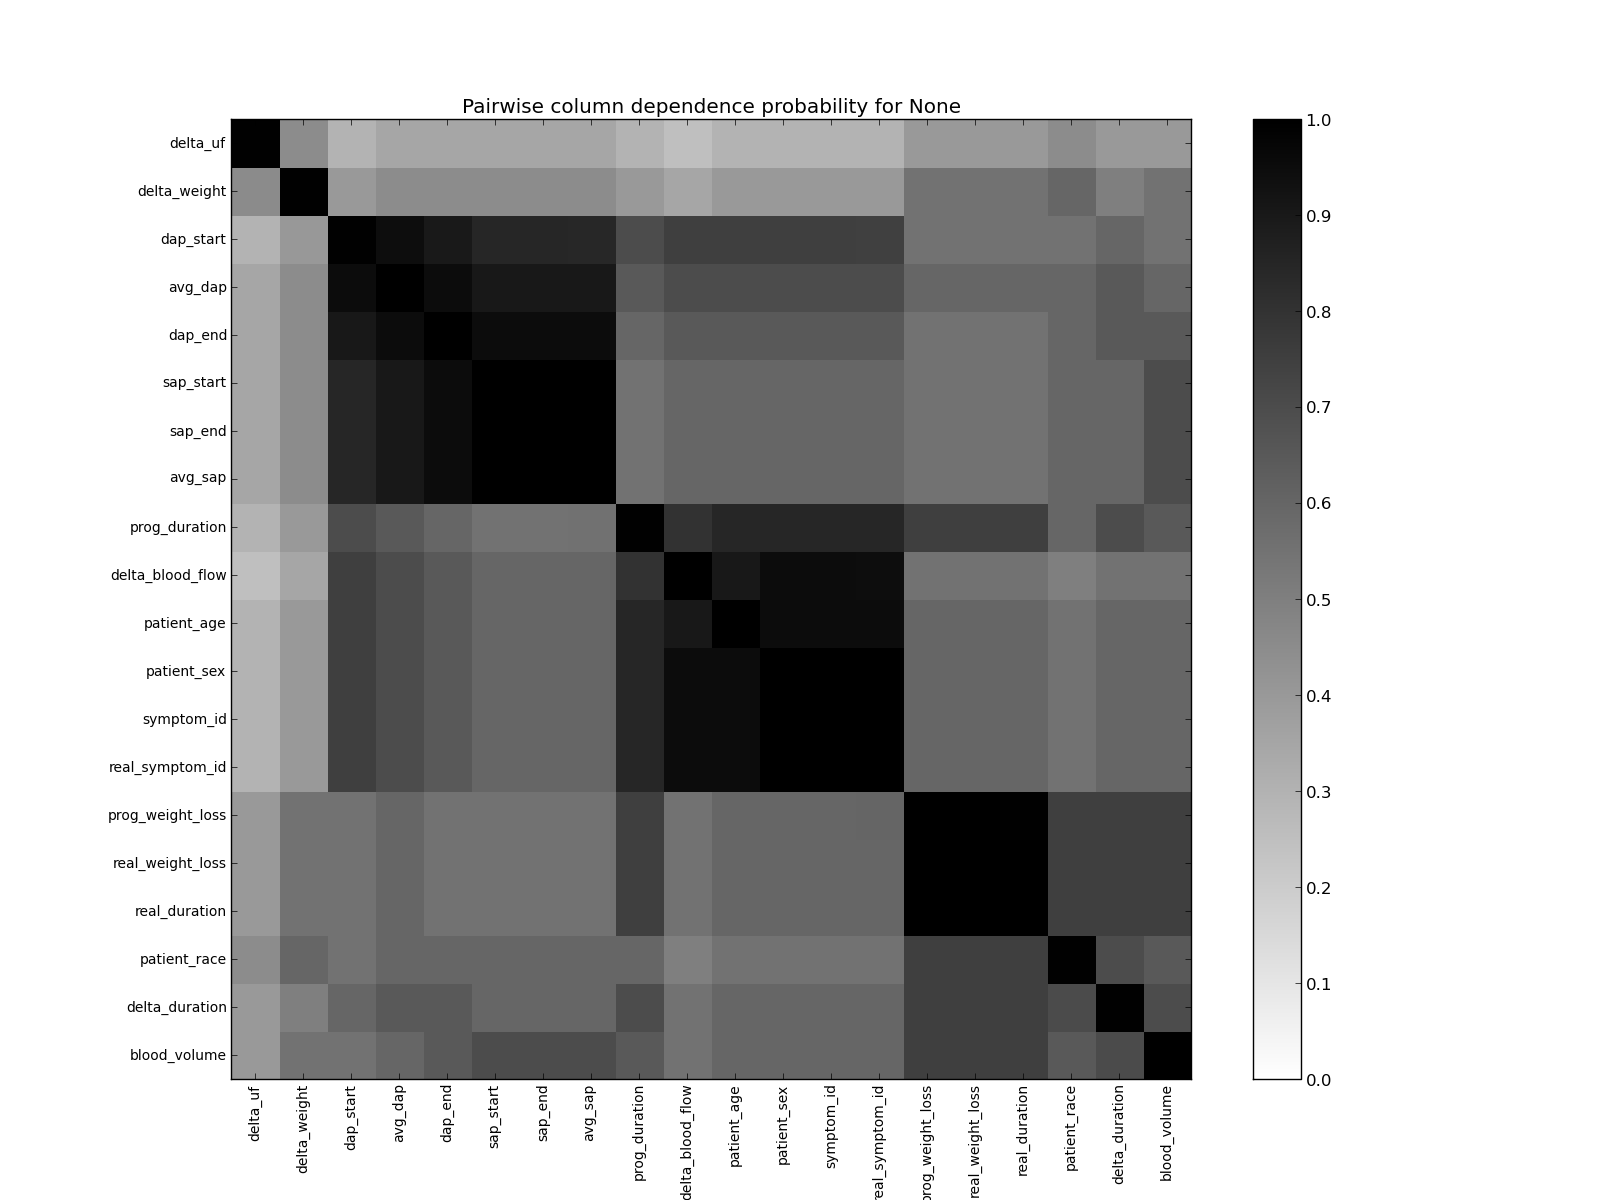
\includegraphics[width=250pt]{../bayesdb/dialysis_prob_dependencies.png}
\caption{Probabilit\'a di dipendenza fra gli attributi}
\label{fig:bayesdb-dep-prob1}
\end{figure}

Essendo interessati esclusivamente alle dipendenze fra la sintomatologia e tutti gli altri attributi, si raffina la \textit{query} precedente:
\begin{verbatim}
ESTIMATE DEPENDENCE PROBABILITIES FROM dialysisai
REFERENCING symptom_id WITH CONFIDENCE 0.9;
\end{verbatim}
che restituisce l'immagine in figura \ref{fig:bayesdb-dep-prob2}; questa mostra solo gli attributi con una evidente una dipendenza della sintomatologia, quali differenza del flusso del sangue, età e sesso (ignorando la banale dipendenza con \verb|real_symptom_id|).

\begin{figure}[!htb]
\centering
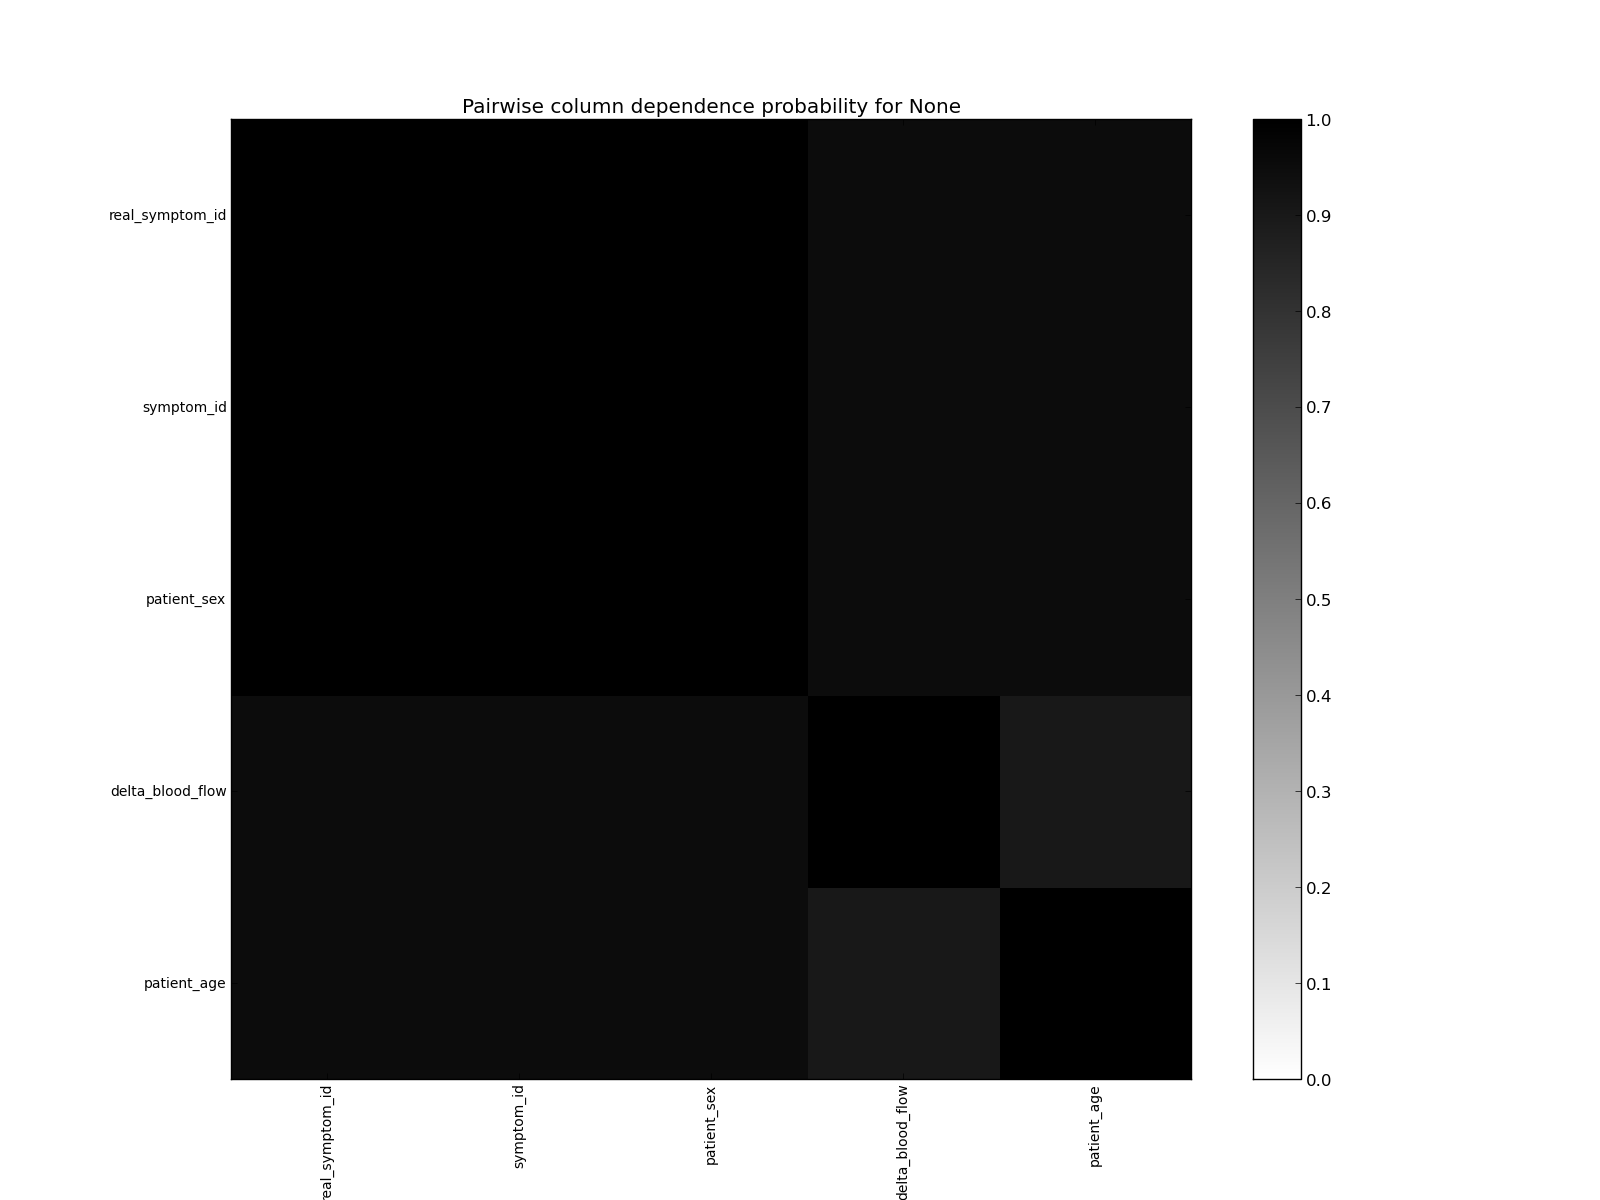
\includegraphics[width=250pt]{../bayesdb/dialysis_prob_dependencies_symptom.png}
\caption{Probabilit\'a di dipendenza fra sintomo e gli altri attributi}
\label{fig:bayesdb-dep-prob2}
\end{figure}

\paragraph{Predizione del sintomo}
Per predire la sintomatologia per ogni record non classificato, si pu\'o eseguire la \textit{query}:
\begin{verbatim}
INFER symptom_id
FROM dialysisai
WITH CONFIDENCE 0.9;
\end{verbatim}

Il risultato restituito a video \'e la lista di tutte le predizioni dei valori di sintomatologia: dove il valore \'e stato predetto, esso \'e preceduto da un asterisco \verb|*|, altrimenti viene mostrato il valore pre-esistente.

\paragraph{Test e risultati}
Il Bayesian Query Language (BQL), linguaggio alla base di BayesDB, non \'e ancora del tutto completo\footnote{La versione utilizzata \'e la \verb|0.1.0 alpha|.}, pertanto non permette una veloce aggregazione dei risultati (conteggi, medie, ecc.).\\
Per questa ragione, \'e stato creato uno script Python\footnote{Lo script \'e \verb|bayesdb/learn_data_test.py|.} che, una volta avviato, stampa a video e su file\footnote{Il log avr\'a il nome \verb|learn_data_test.log|.} il risultato dei test sulla predizione effettuata.

La query eseguita seleziona il sintomo vero, che non verr\'a modificato poich\'e sempre presente, e il sintomo da predire, che sar\'a inferito dal sistema con un livello di confidenza di $0.9$\footnote{Il valore inferito viene solo caricato e mostrato a video, la base di dati non viene modificata.}.
\begin{verbatim}
INFER real_symptom_id, symptom_id 
FROM dialysisai
WITH CONFIDENCE 0.9;
\end{verbatim}

Quindi, lo script procede ad analizzare i dati restituiti dalla query, calcolando \textit{true positive rate}, \textit{false positive rate}, \textit{precision}, \textit{recall} e F-Measure, mostrate in tabella \ref{table:risultati-bayesdb}.

\begin{table}[h]
\centering
\begin{tabular}{|r|l|} \hline
\multicolumn{2}{|c|}{\textbf{BayesDB}} \\ \hline \hline 
\textbf{+} & $100$ \\ \hline
\textbf{TPR} & $0.90$ \\ \hline
\textbf{FPR} & $0.01$ \\ \hline
\textbf{Precision} & $0.98$ \\ \hline
\textbf{Recall} & $0.90$ \\  \hline
\textbf{F-Measure} & $0.94$ \\
\hline\end{tabular}
\caption{Risultato di esecuzione di BayesDB}
\label{table:risultati-bayesdb}
\end{table}

\section{Sviluppi futuri}
\label{sviluppi-futuri}
L'implementazione base del C4.5 realizzata \'e migliorabile in molti punti.

Un primo miglioramento potrebbe riguardare la generazione dinamica dei range degli attributi: la cardinalit\'a di ogni range non sarebbe pi\'u fissa, ma varierebbe a seconda della vicinanza dei valori degli esempi o secondo altri criteri.

Come gi\'a detto in \ref{risultati-no-ktv-qb}, sarebbe molto utile eliminare, a fine processo, tutte quelle regole che risultano superflue nel senso che non vanno a includere molti esempi positivi in pi\'u rispetto alle altre; le regole, quindi, potrebbero risultare anche pi\'u compatte.

Inoltre, si potrebbe confrontare la precisione del programma nel caso i valori nulli non vengano riempiti ``a monte'' del processo (ovvero nel database), e vengano quindi ignorati completamente.

Ad oggi, il programma gestisce gli esempi come strettamente positivi o negativi. Avendo a disposizione circa $60$ sintomi, tuttavia, potrebbe risultare utile riadattare alcune parti dell'algoritmo con il fine di classificare, in un unico albero di decisione, tutti i sintomi. Un possibile svantaggio si potrebbe avere relativamente a sintomi che hanno pochi esempi che li soddisfano, e che potrebbero non essere rappresentati da nessuna regola generata. Ci sarebbe, in questo caso, anche da valutare il costo dell'algoritmo, sicuramente pi\'u complesso (si veda il calcolo dell'entropia).

Infine, vista la scarsa distribuzione delle sintomatologie per seduta di dialisi, potrebbe essere utile imporre una certa soglia di tolleranza, ad esempio andando a classificare come nodo foglia anche i nodi che contengono esempi positivi in una certa percentuale ($95\%$ anzich\'e $100\%$ come attualmente implementato). In questo modo sarebbe anche possibile definire un ordine di priorit\'a per le regole generate, da quella ``pi\'u certa'' a quella con la pi\'u bassa probabilit\'a.

Miglioramenti implementativi potrebbero essere:
\begin{itemize}
\item personalizzazione del numero dei \textit{fold} da utilizzare nella $k$\textit{-fold cross-validation}
\item spostamento dell'intero processo di apprendimento su macchine virtuali nel cloud; \'e gi\'a in studio una migrazione su Google Compute Engine
\item apprendimento multi-threading sui diversi split dei $k$\textit{-fold}
\item apprendimento multi-threading sui diversi \textit{range} dell'attributo migliore ad ogni livello dell'albero 
\item eliminazione di regole troppo lunghe o che classificano pochi elementi (necessario un set esterno di validazione)
\item ordinamento delle regole in base all'\textit{error rate} del passo in cui sono state apprese (diretta proporzionalit\'a tra ordine regola e ordine \textit{error rate}) e alla loro semplicit\'a (minor numero di clausole, maggiore rilevanza)
\end{itemize}

\bibliographystyle{abbrv} % standard abbrv style
\bibliography{bibliography}

\appendix

\section{Importazione dei dati}
\label{appendix-data}
Per utilizzare il database come sorgente dei dati, occorre installare \href{http://www.mysql.com/}{MySQL} come motore di database.
Quindi:

\begin{enumerate}
\item Avviare il server MySQL.
\item Tramite il tool "Import Data" di MySQL Workbench, selezionare il file \verb|scripts/mysq-dump.sql| e avviare l'importazione dei dati.
\item Avviare lo script \verb|scripts/mysql-scores.sql| per la creazione delle \textit{view} utili.
\end{enumerate}

\section{Setup di Weka}
\label{appendix-weka}
Per utilizzare Weka con i file ARFF, localizzati nella cartella \verb|weka/|, non serve nessun pre-requisito particolare. Per la connessione al database, invece, serve specificare il file \verb|DatabaseUtils.props| che contiene alcune propriet\'a per la connessione.

Un file di esempio \'e \verb|weka/DatabaseUtils.props|, che permette di collegarsi a fonti dati MySQL. In particolare, le informazioni rilevanti da gestire sono:
\begin{verbatim}
# JDBC driver (comma-separated list)
jdbcDriver=com.mysql.jdbc.Driver,
  org.gjt.mm.mysql.Driver

# database URL
jdbcURL=jdbc:mysql://localhost:3306/DialysisAI
\end{verbatim}

Successivamente serve includere, se non gi\'a presente, la libreria \verb|jar| per le connessioni JDBC ai database MySQL nel \textit{classpath} caricati da Weka.
Ad esempio, su Windows serve modificare il file \verb|RunWeka.ini| (presente nel percorso di installazione di Weka) in modo tale che la variabile \verb|cp| includa, all'ultima riga, il percorso completo del file \verb|jar|:
\begin{verbatim}
cp=%CLASSPATH%;%MY_SQL_PATH%/Connector J 5.1.29/
  mysql-connector-java-5.1.29-bin.jar
\end{verbatim}

\section{BayesDB}

\subsection{Installazione di BayesDB}
\label{appendix-bayesdb}
Per avviare una versione funzionante di BayesDB, si suggerisce di utilizzare la VirtualBox VM messa a disposizione sul \href{http://probcomp.csail.mit.edu/bayesdb/#Download}{sito ufficiale}, in quanto contiene una versione gi\'a configurata e pronta all'uso.\\
All'avvio della VM, \'e possibile utilizzare BayesDB, essendo avviato in automatico.

\subsection{Collegamento alla VM}
\label{appendix-bayesdb-collegamento}
La macchina virtuale su cui BayesDB \'e preinstallato non supporta la configurazione di tastiera italiana; pertanto \'e conveniente accedere alla \textit{shell} Ubuntu tramite protocollo SSH.

Su sistemi Linux/Mac OS X, digitare in una shell:
\begin{verbatim}
$ ssh -i vm_guest_id_rsa -p 2222 
  -o StrictHostKeyChecking=no bayesdb@localhost
\end{verbatim}

Su sistemi Windows, \verb|ssh| \'e incluso nella distribuzione di \href{http://git-scm.com/}{Git}.

\subsection{Trasferimento da e verso BayesDB}
\label{appendix-bayesdb-trasferimento}
Per inviare file dalla macchina locale alla VM (e viceversa), utilizzare l'eseguibile \verb|scp| (secure \verb|cp|).

Su sistemi Linux/Mac OS X, digitare in una shell:
\begin{verbatim}
$ scp -r -i vm_guest_id_rsa -p 2222 
  -o StrictHostKeyChecking=no 
  path/to/file bayesdb@localhost:/home/bayesdb/file
\end{verbatim}

Su Windows, installare \href{http://winscp.net/eng/index.php}{WinSCP} e configurarlo con i seguenti parametri:
\begin{itemize}
\item server: \verb|localhost|
\item port: \verb|2222|
\item username: \verb|bayesdb|
\item password: \verb|bayesdb|
\item key: utilizzare la chiave \verb|vm_guest_id_rsa|, fornita nel pacchetto della VirtualBox VM scaricato dal sito di BayesDB (ignorare gli avvisi di incompatibilit\'a della chiave con Putty)
\end{itemize}

\subsection{Esecuzione di query}
\label{appendix-bayesdb-query}
Dopo aver fatto accesso alla VM in SSH, aprire una console Python digitando il comando \verb|python|, e ottenere un'istanza del client BayesDB:
\begin{verbatim}
>>> from bayesdb.client import Client
>>> client = Client()
\end{verbatim}
A questo punto, si pu\'o utilizzare \verb|client| per eseguire qualsiasi \textit{query}, ad esempio:
\begin{verbatim}
>>> client('INFER real_symptom_id, symptom_id '
...     'FROM dialysisai '
...     'WITH CONFIDENCE 0.9;')
\end{verbatim}

\balancecolumns

% That's all folks! % GM Sept. 2008
\end{document}
